
\chapter{$\eta \eta \to h h$}

Author:  Wady Alexander Ríos Herrera

Proceso: \textbf{Radiative seesaw II}\\

Experimentos de reactores  de neutrinos han demostrado que los neutrinos tienen masa.


\section{Lagrangian}


El modelo considerado es una extensión del modelo estándar, el contiene SU($2$)$\times$ U($1$)$_{Y}$ de singletes $N_{i}$ y un segundo doblete de Higgs $\eta$. En adición, una simetría discreta exacta $Z_{2}$ es asumida tal que el nuevo campo son impares bajo $Z_{2}$, mientras que en el modelo estándar son pares. El lagrangiano de interacción de  Yukawa inducido por el nuevo doblete Higgs es dada por  \cite{1}
\begin{equation}
L_{Y}=\epsilon _{ab}h_{\alpha j}\bar{N}_{j}P_{L}L_{\alpha}^{a}\eta ^{b}+H.c,
\label{1}
\end{equation}
 
L son doblete de leptón izquierdo, $\alpha , j$ son indices de generación (Greek indices etiquetado sabor leptonico e,$\mu$,$\tau$) y $\epsilon _{ab}$ es el tensor antisimetrico completo.\\

A partir del lagrangiano de interacción de Yukawa se determina el langrangiano interacción escalar cuadrático  \cite{2} 

\begin{equation}
L_{I}=\lambda_{3}(\Phi^{+}\Phi)( \eta^{+}\eta)+\lambda_{2}(\Phi^{+}\eta)( \eta^{+}\Phi) \frac{\lambda _{5}}{2}(\Phi^{+}\eta + H.C)
\label{2}
\end{equation}


Donde $\Phi$ es el modelo estándar del doblete de Higgs y es solo relevante para generación de masa neutrina. Ya que $Z_{2}$ es asumida  ser  exactamente simétrica del modelo $\eta$ tiene valor esperado del vacío cero. La Física escalar de los bosones son por lo tanto $R_{e}\Phi ^{0},\eta^{\pm},\eta_{0}^{R}\equiv Re\eta_{0}, \eta_{0}^{I}\equiv Im\eta_{0} =0 $ y $Im\eta^{+} =0$.\\


para ecuación \ref{2} se tiene que 
\begin{equation}
\Phi=\begin{pmatrix}
0 & \frac{h+v}{\sqrt{2}}
\end{pmatrix}, \ \eta= \begin{pmatrix}
\eta^{+} & \\
\eta_{0} & 
\end{pmatrix} 
\label{2.1}
\end{equation}

donde $h$ y $v$ son parámetros reales por tanto $\Phi =\Phi ^{+}$


Remplazando \ref{2.1} y las partes reales de $\eta$ el lagrangiano \ref{2} se determina el termina el termino relevante

\begin{equation*}
L_{I}=\lambda_{l} \left[\begin{pmatrix}
0 & \frac{h+v}{\sqrt{2}}
\end{pmatrix}\begin{pmatrix}
\eta^{+} & \\
\eta_{0} & 
\end{pmatrix}\right]^{2}= \lambda_{l}\left[0\eta^{+}+\left( \frac{h+v}{\sqrt{2}}\right)\eta_{0}\right]^{2}
\end{equation*}
\begin{equation*}
=\lambda_{l}(h+v)^{2}(\eta_{0})^{2}=\lambda_{l}(h^{2}+2hv+v^{2})(\eta_{0})^{2}
\end{equation*}
\begin{equation}
=\underbrace{\lambda_{l}h^{2}\eta_{0}^{2}}_{\star}+2\lambda_{l}hv\eta_{0}^{2}+\lambda_{l}v^{2}\eta_{0}^{2}, 
\label{3}
\end{equation}

Con 
\begin{equation}
\lambda_{l}=\frac{\lambda _{3}+\lambda _{4}+\lambda _{5}}{2}
\end{equation}

donde el termino relevante de la expresión \ref{3} es denotado con $\star$, ya que este genera el siguiente proceso 

\begin{figure*}[htb]
    \centering
    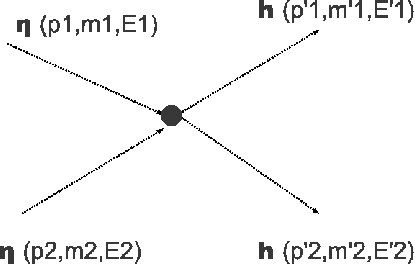
\includegraphics[width=0.5\textwidth]{1}%(eps preferiblemente)
    \caption[electrones]{Proceso donde dos etas se destruyen y se crean dos Higgs}
    \label{fi}
\end{figure*}
 



Por tanto el lagrangiano de interés es
\begin{equation}
L_{i}=\lambda_{l}h^{2}\eta_{0}^{2}
\label{4}
\end{equation}










\section{S-matriz}
 El orden a calcular la matriz $S$ es de orden uno ya que solo tenemos un termino de interacción \ref{4} el cual  determina el proceso de figuara \ref{fi}.\\
 Consideremos el proceso de la figura \ref{fi} donde $\eta(p_{1})\eta(p_{2})$ decae a un par de $h(p_{1}^{'})h(p_{2}^{'})$.
 El elemento de matriz $S_{fi}^{1}$ entre el estado inicial  y el estado final es 
 
 \begin{equation}
S_{fi}^{(1)}=-\lambda_{l}\int d^{4}x\bra{h(p_{1}^{'})h(p_{2}^{'})}h^{2}\eta_{0}^{2}\ket{\eta(p_{1})\eta(p_{2})}, 
 \label{5}
 \end{equation}
 
 sabemos que
 
 \begin{equation}
\eta_{0}=\eta_{+}+\eta_{-}=\frac{1}{\sqrt{2E_{p}V}}\left[ae^{-ip.x}+a^{+}e^{ip.x}\right]
 \label{6}
 \end{equation}

\begin{equation}
h=h_{+}+h_{-}=\frac{1}{\sqrt{2E_{p}V}}\left[ae^{-ip.x}+a^{+}e^{ip.x}\right]
 \label{7}
 \end{equation}


Por lo tanto
\begin{equation*}
h^{2}=\left(h_{+}+h_{-}\right)^{2}=(h_{+}+h_{-})(h_{+}+h_{-})
\end{equation*}
 \begin{equation}
=h_{+}h_{+}+h_{+}h_{-}+h_{-}h_{+}+h_{-}h_{-}
 \label{8}
 \end{equation}

\begin{equation*}
\eta_{0}^{2}=\left(\eta_{+}+\eta_{-}\right)^{2}=(\eta_{+}+\eta_{-})(\eta_{+}+\eta_{-})
\end{equation*}
\begin{equation}
=\eta_{+}\eta_{+}+\eta_{+}\eta_{-}+\eta_{-}\eta_{+}+\eta_{-}\eta_{-}
\label{9}
\end{equation}

El termino $\frac{1}{\sqrt{2E_{p}V}}$ de la expresión \ref{6} y \ref{7} es de normalización.\\

Calculemos  el termino $h^{2}\eta_{0}^{2}$:
\begin{equation*}
h^{2}\eta_{0}^{2}=(h_{+}h_{+}+h_{+}h_{-}+h_{-}h_{+}+h_{-}h_{-})(\eta_{+}\eta_{+}+\eta_{+}\eta_{-}+\eta_{-}\eta_{+}+\eta_{-}\eta_{-})
\end{equation*}
\begin{equation*}
=h_{+}h_{+}\eta_{+}\eta_{+}+h_{+}h_{+}\eta_{+}\eta_{-}+h_{+}h_{+}\eta_{-}\eta_{+}+h_{+}h_{+}\eta_{-}\eta_{-}+
\end{equation*}
\begin{equation*}
h_{+}h_{-}\eta_{+}\eta_{+}+h_{+}h_{-}\eta_{+}\eta_{-}+h_{+}h_{-}\eta_{-}\eta_{+}+h_{+}h_{-}\eta_{-}\eta_{-}+
\end{equation*}
\begin{equation*}
h_{-}h_{+}\eta_{+}\eta_{+}+h_{-}h_{+}\eta_{+}\eta_{-}+h_{-}h_{+}\eta_{-}\eta_{+}+h_{-}h_{+}\eta_{-}\eta_{-}+
\end{equation*}
\begin{equation}
h_{-}h_{-}\eta_{+}\eta_{+}+h_{-}h_{-}\eta_{+}\eta_{-}+h_{-}h_{-}\eta_{-}\eta_{+}+h_{-}h_{-}\eta_{-}\eta_{-}
\label{10}
\end{equation}
 Por otro lado  sabemos que 
 
 \begin{equation}
 h_{+}\ket{h}=\frac{1}{\sqrt{2E_{p}V}}e^{-ip.x}\ket0 ,\ h_{-}\ket{h}=\frac{1}{\sqrt{2E_{p}V}}e^{ip.x}\ket{1_{h}}
 \label{11}
 \end{equation}
 \begin{equation}
 \bra h h_{-}=\frac{1}{\sqrt{2E_{p}V}}e^{ip.x}\bra{0} ,\ \bra h h_{+}=\frac{1}{\sqrt{2E_{p}V}}e^{-ip.x}\bra{1_{h}}
 \label{12}
 \end{equation}


\begin{equation}
 \eta_{+}\ket{\eta}=\frac{1}{\sqrt{2E_{p}V}}e^{-ip.x}\ket0 ,\ \eta_{-}\ket{\eta}=\frac{1}{\sqrt{2E_{p}V}}e^{ip.x}\ket{1_{\eta}}
 \label{13}
 \end{equation}
 \begin{equation}
 \bra \eta \eta_{-}=\frac{1}{\sqrt{2E_{p}V}}e^{ip.x}\bra{0} ,\ \bra \eta \eta_{+}=\frac{1}{\sqrt{2E_{p}V}}e^{-ip.x}\bra {1_{\eta}}
 \label{14}
 \end{equation}
 
 y
 
 \begin{equation}
\bra{h(p_{1}^{'})h(p_{2}^{'})}h_{+}h_{+}=\frac{1}{\sqrt{2E_{p_{1}^{'}}V}}\frac{1}{\sqrt{2E_{p_{2}^{'}}V}}e^{-ip_{1}^{'}.x}e^{-ip_{2}^{'}.x}\bra{1_{h}1_{h}}
 \label{15}
 \end{equation}
\begin{equation}
\bra{h(p_{1}^{'})h(p_{2}^{'})}h_{+}h_{-}=\frac{1}{\sqrt{2E_{p_{1}^{'}}V}}\frac{1}{\sqrt{2E_{p_{2}^{'}}V}}e^{-ip_{1}^{'}.x}e^{ip_{2}^{'}.x}\bra{1_{h}0}
 \label{16}
 \end{equation}
\begin{equation}
\bra{h(p_{1}^{'})h(p_{2}^{'})}h_{-}h_{+}=\frac{1}{\sqrt{2E_{p_{1}^{'}}V}}\frac{1}{\sqrt{2E_{p_{2}^{'}}V}}e^{ip_{1}^{'}.x}e^{-ip_{2}^{'}.x}\bra{01_{h}}
 \label{17}
 \end{equation}
\begin{equation}
\bra{h(p_{1}^{'})h(p_{2}^{'})}h_{-}h_{-}=\frac{1}{\sqrt{2E_{p_{1}^{'}}V}}\frac{1}{\sqrt{2E_{p_{2}^{'}}V}}e^{ip_{1}^{'}.x}e^{ip_{2}^{'}.x}\bra{00}
 \label{18}
 \end{equation}

\begin{equation}
\eta_{+}\eta_{+}\ket{\eta(p_{1})\eta(p_{2})}=\frac{1}{\sqrt{2E_{p_{1}}V}}\frac{1}{\sqrt{2E_{p_{2}}V}}e^{-ip_{1}.x}e^{-ip_{2}.x}\ket{00}
 \label{19}
 \end{equation}


\begin{equation}
\eta_{+}\eta_{-}\ket{\eta(p_{1})\eta(p_{2})}=\frac{1}{\sqrt{2E_{p_{1}}V}}\frac{1}{\sqrt{2E_{p_{2}}V}}e^{-ip_{1}.x}e^{ip_{2}.x}\ket{01_{\eta}}
 \label{20}
 \end{equation}
\begin{equation}
\eta_{-}\eta_{+}\ket{\eta(p_{1})\eta(p_{2})}=\frac{1}{\sqrt{2E_{p_{1}}V}}\frac{1}{\sqrt{2E_{p_{2}}V}}e^{ip_{1}.x}e^{-ip_{2}.x}\ket{1_{\eta}0}
 \label{21}
 \end{equation}
\begin{equation}
\eta_{-}\eta_{-}\ket{\eta(p_{1})\eta(p_{2})}=\frac{1}{\sqrt{2E_{p_{1}}V}}\frac{1}{\sqrt{2E_{p_{2}}V}}e^{ip_{1}.x}e^{ip_{2}.x}\ket{1_{\eta}1_{\eta}}
 \label{22}
 \end{equation}

Por tanto san duchando el termino $h^{2}\eta_{0}^{2}$ con las relaciones desde \ref{15} hasta \ref{22} el termino que sobrevive es


\begin{equation*}
\bra{h(p_{1}^{'})h(p_{2}^{'})}h^{2}\eta_{0}^{2}\ket{\eta(p_{1})\eta(p_{2})}=\bra{h(p_{1}^{'})h(p_{2}^{'})}h_{-}h_{-}\eta_{+}\eta_{+}\ket{\eta(p_{1})\eta(p_{2})}
\end{equation*}
\begin{equation}
=\frac{1}{\sqrt{2E_{p_{1}^{'}}V}}\frac{1}{\sqrt{2E_{p_{2}^{'}}V}}\frac{1}{\sqrt{2E_{p_{1}}V}}\frac{1}{\sqrt{2E_{p_{2}}V}}e^{i(p_{1}^{'}+p_{2}^{'}-p_{1}-p_{2})}\bra{00}\ket{00}
\label{23}
\end{equation}

remplazando \ref{23} en matriz $S_{fi}^{(1)}$ obtenemos

\begin{equation}
S_{fi}^{(1)}=-i\lambda_{l}\frac{1}{\sqrt{2E_{p_{1}^{'}}V}}\frac{1}{\sqrt{2E_{p_{2}^{'}}V}}\frac{1}{\sqrt{2E_{p_{1}}V}}\frac{1}{\sqrt{2E_{p_{2}}V}}\int d^{4}x e^{i(p_{1}^{'}+p_{2}^{'}-p_{1}-p_{2})}\bra{00}\ket{00}
\label{24}
\end{equation}


El valor de la integral es $(2\pi)^{4}\delta^{4}(p_{1}+p_{2}-p_{1}^{'}-p_{2}^{'})$ y $\bra{00}\ket{00}=1$ por tanto el elemento de matriz obtenido es

\begin{equation}
S_{fi}^{(1)}=-i\lambda_{l}\frac{1}{\sqrt{2E_{p_{1}^{'}}V}}\frac{1}{\sqrt{2E_{p_{2}^{'}}V}}\frac{1}{\sqrt{2E_{p_{1}}V}}\frac{1}{\sqrt{2E_{p_{2}}V}}(2\pi)^{4}\delta^{4}(p_{1}+p_{2}-p_{1}^{'}-p_{2}^{'})
\label{25}
\end{equation}



\section{Process calculation}

 De la ecuación \ref{25} la función $\delta$  es la conservación de los $4$-momentos en el proceso general, el cual es multiplicado por $(2\pi)^{4}$. Hay un factor $(2EV)^{\frac{-1}{2} }$ para cada partícula del estado inicial y del estado final de energía $E$. El restos de termino de la expresión \ref{25} el cual depende sobre la naturaleza exacta de la interacción es llamada la amplitud de Feynman, es denotada por $iM_{fi}$.\\
 Para nuestro caso  
 \begin{equation}
iM_{fi}= -i\lambda_{l}
  \label{26}
 \end{equation}
              
   Para determinar la sección eficaz de nuestro modelo se determina a partir de expresión\cite{3}
   
   \begin{equation}
\frac{d\sigma}{d\Omega}=\frac{1}{64 \small{\pi} ^{2}s}\left[\frac{(s-(m_{1}^{'}+m_{2}^{'})^{2})(s-(m_{1}^{'}-m_{2}^{'})^{2}))}{(s-(m_{1}+m_{2})^{2})(s-(m_{1}-m_{2})^{2}))}\right]^{\frac{1}{2}}\overline{\vert M_{fi}\vert^{2}}
   \label{27}
   \end{equation}            
              
     Donde $m_{1}^{'}=m_{2}^{'}=m_{h}$ es la masa del Higgs, $m_{1}=m_{2}=m_{\eta}$ es la masa del eta y  $\overline{\vert M_{fi}\vert^{2}}=\lambda_{l}$ es la amplitud de Feynman, remplazando estos términos en la expresión \ref{27} se obtiene
     
     \begin{equation}
      \frac{d\sigma}{d\Omega}=\frac{1}{64\small{\pi} ^{2}s}\left[\frac{(s-4m_{h}^{2})}{(s-4m_{\eta}^{2})}\right]^{\frac{1}{2}}\left(\lambda_{l}\right)^{2}
          \label{28}
     \end{equation}
     
     
Con $s=\sqrt{E_{1}+E_{2}}$ y $E=\sqrt{p^{2}+m^{2}}$, la integral sobre $d\Omega$ es $4\pi$ por tanto la sección eficaz es 


\begin{equation}
  \sigma=\frac{(\lambda_{l})^{2}}{64\small{\pi} s}\left[\frac{(s-4m_{h}^{2})}{(s-4m_{\eta}^{2})}\right]^{\frac{1}{2}}
  \label{29}
\end{equation}  
          
     
     
Para determinar un valor númerico de la sección eficaz tomamos los siguientes valores: $ m_{\eta}=50GeV, m_{h}=120 GeV, \lambda_{l}=0.1$ y $\sqrt{s}=1016.68GeV $, Por tanto la expresión \ref{29} que así

\begin{equation*}
\sigma=\frac{(0.1)^{2}}{64\small{\pi} (1016.68GeV)^{2}}\left[\frac{(1016.68GeV)^{2}-4(120GeV)^{2}}{(1016.68GeV)^{2}-4(50GeV)^{2}}\right]^{\frac{1}{2}}
\label{30}GeV
\end{equation*}
     \begin{equation*}
    \frac{(0.1)^{2}}{64\small{\pi} (1016.68GeV)^{2}}\left[\frac{976055.3134 (GeV)^{2}}{1023638.232(GeV)^{2}}\right]^{\frac{1}{2}}
     \end{equation*}
              
\begin{equation*}
   = \frac{(0.1)^{2}}{64\small{\pi} (1016.68GeV)^{2}}(0,9764)
     \end{equation*}   
     \begin{equation}
    =4,69\times 10^{-11}(GeV)^{-2}
     \end{equation}              
              
\section{CalcHEP comparison}
Para ser la simulación se instala los programas de LanHep y CalHep.\\
Después se baja los archivos del proceso a simular de github, nuestro archivo pertinente es la carpeta idm para nuestro sistema. Se  instala la carpeta idm  en LanHep y CalHep y se ejecuta  CalHep desde el directorio idm para iniciar la simulación.\\
Los parámetros de la simulación son $~H0,~H0->H,H$ donde se descoge el diagrama de la figura \ref{fi} luego se ingresa los parámetros de la simulación que son $\lambda_{l}=0.1, m_{\eta}=50 GeV, m_{h}=120 GeV$, momento inicial $500 GeV$ y momento final es de $500GeV$ por tanto al sección eficaz de la simulación es de $0.145983[pb]$  

\section{Copyright}

\includegraphics[scale=0.5]{cc} Creative Commons Attribution-Share Alike 3.0 United States License.

\begin{thebibliography}{9}

\bibitem{1} D. Aristizabal Sierra, Jisuke Kubo and Daijiro Suematsu, Physical Review D 79, 013001 (2009)
\bibitem{2} Ernast Ma, Physical Review D 73, 0077301(2006)
\bibitem{3} Quantum Fiel Theory, Amitabha Lahiri and Palash B. Pal

\end{thebibliography}

%%% Local Variables: 
%%% mode: latex
%%% TeX-master: "qft_samples"
%%% End: 
